\section{Introduzione}

La \textit{data inference} è lo studio dei metodi che utilizzano i dati per predirre il futuro. 
Il \textit{Machine Learning} è uno strumento potente che può essere usato per risolvere una 
grossa parte dei problemi di \textit{data inference}, inclusi i seguenti:
\begin{itemize}
    \item \textbf{Clustering}: raggruppare i \textit{data points} in base alle loro similarità;
    \item \textbf{Prediction}: assegnare delle etichette (\textit{label}) ai \textit{data points};
    \item \textbf{Generation}: generare nuovi \textit{data points};
    \item    \textbf{Control}: eseguire una sequenza di azioni in un ambiente con l'obiettivo di
                               massimizzare una nozione di utilità.
\end{itemize}

Con \textit{data point} si intende una serie di informazioni legate ad un unico elemento;
un'analogia può essere un \textit{record} in un database.

Gli algoritmi che risolvono una \textit{learning task} in base a dei dati già semanticamente
etichettati lavorano in modalità \textbf{\textit{supervised learning}}. A etichettare i dati
saranno delle persone o la natura. Un esempio dell'ultimo caso sono le previsioni del meteo. 
D'altra parte, gli algoritmi che utilizzano i dati senza la presenza di etichette lavorano in
modalità \textbf{\textit{unsupervised learning}}.

In questo corso ci si focalizzerà sul \textit{supervised learning} e la progettazione di 
sistemi di \textit{machine learning} il cui obiettivo è apprendere dei 
\textbf{predittori}, ovvero funzioni che mappano i \textit{data points} alla loro
etichetta.

\subsection{Label set \texorpdfstring{$\Y$}{Y}}
Verrà usata $\Y$ per indicare il label set, ovvero l'insieme di tutte le possibili
etichette di un \textit{data point}. Le etichette potranno essere di due tipi differenti:
\begin{enumerate}
    \item \textbf{Categoriche} ($\Y = \{ \text{sport},\text{politica},\text{economia}\}$):
        si parlerà di problemi di \textbf{classificazione};
    \item \textbf{Numeriche} ($\Y \subseteq \mathbb{R} $): 
        si parlerà di problemi di \textbf{regressione}.
\end{enumerate}

È importante sottolineare come la reale differenza tra le due tipologie di etichetta sia il
significato e non la sua rappresentazione in quanto, si potrà sempre codificare
un'etichetta categorica in un numero.

A sottolineare ciò è il fatto che nella regressione l'errore è tipicamente una funzione della
differenza $| y-\hat{y} |$, dove $\hat{y}$ è la predizione di $y$. Nella classificazione, invece,
l'errore è tipicamente binario: predizione corretta ($\hat{y}=y$) o errata ($\hat{y}\neq y$).

Quando ci sono solo due possibili etichette ($|\Y|=2$), si ha un \textbf{problema di 
classificazione binario} e, convenzionalmente, verrà usata una codifica numerica 
$\Y=\{-1,1\}$.

\subsection{Loss function \texorpdfstring{$\loss$}{l}}
Come già visto precedentemente, si vuole misurare l'errore che un predittore commette su una
determinata predizione. Per farlo si userà una \textbf{funzione di loss} $\loss$ non negativa 
che misurerà la discrepanza $\loss(y,\hat{y})$ tra l'etichetta predetta $\hat{y}$ e quella
corretta $y$. Si assumerà sempre $\loss(y,\hat{y})=0$ quando $\hat{y}=y$.

La funzione di loss più semplice per la classificazione è la \textbf{zero-one loss}:
$$ \loss(y,\hat{y}) = \begin{cases} 0 & y=\hat{y} \\ 1 & \text{altrimenti} \end{cases} $$

Nella regressione, le tipiche funzioni di loss sono:
\begin{itemize}
    \item la \textit{\textbf{absolute loss}}: $\loss(y,\hat{y}) = |y-\hat{y}|$
    \item la \textit{\textbf{quadratic loss}}: $\loss(y,\hat{y}) = (y-\hat{y})^2$
\end{itemize}

In alcuni casi può essere conveniente scegliere l'etichetta predetta da un insieme $\Z$ diverso 
da $\Y$. Per esempio, si consideri il problema di assegnare una probabilità $\hat{y}\in (0,1)$
all'evento $y=\text{\quotes{pioverà domani}}$. In questo caso, $\Y=\{\text{\quotes{piove}},
\text{\quotes{non piove}}\}$ e $\Z = (0,1)$. Indicando questi due eventi con 1 (piove) e 0 
(non piove), si può usare una funzione di loss per la regressione, come la 
\textit{absolute loss}:
$$ \loss(y,\hat{y}) = |y-\hat{y}| =  \begin{cases} 1-\hat{y} & y=1 \qquad (\text{piove}) \\
\hat{y} & y=0 \qquad (\text{non piove}) \end{cases} $$

Per penalizzare maggiormente le predizioni che distano troppo dalla realtà, si può usare una
\textit{\textbf{logarithmic loss}}:
$$ \loss(y,\hat{y}) = \begin{cases} \ln{\frac{1}{\hat{y}}} & y=1 \qquad 
(\text{piove}) \\ \ln{\frac{1}{1-\hat{y}}} & y=0 \qquad (\text{non piove}) \end{cases} $$

\begin{figure}[h]
    \centering
    \begin{subfigure}{.43\textwidth}
        \centering
        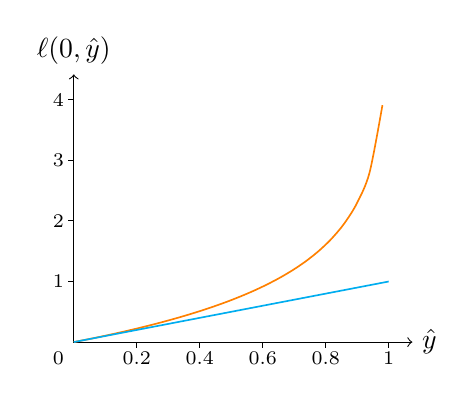
\begin{tikzpicture}

    \draw[<->] (4.3,0) node[right]{$\hat{y}$} -|(0,3.4) node[above]{$\ell(0,\hat{y})$};
    \draw[domain=0:0.98, semithick, smooth, orange] plot ({\x*4},{ln(1/(1-\x))/1.3});
    \draw[domain=0:1, semithick, cyan] plot ({\x*4},{abs(0-\x)/1.3});

    \node[below left] at (0,0) {\scriptsize 0};
    %xticks
    \foreach \x in {0.2,0.4,...,1} {
        \draw (\x*4,0) -- (\x*4,-.07);
    }
    \node[below] at (0.2*4,0) {\scriptsize 0.2};
    \node[below] at (0.4*4,0) {\scriptsize 0.4};
    \node[below] at (0.6*4,0) {\scriptsize 0.6};
    \node[below] at (0.8*4,0) {\scriptsize 0.8};
    \node[below] at (1*4,0)   {\scriptsize 1};
    %yticks
    \foreach \y in {1,...,4} {
        \draw (0,\y/1.3) -- (-.07,\y/1.3);
    }
    \node[left] at (0,1/1.3) {\scriptsize 1};
    \node[left] at (0,2/1.3) {\scriptsize 2};
    \node[left] at (0,3/1.3) {\scriptsize 3};
    \node[left] at (0,4/1.3) {\scriptsize 4};

\end{tikzpicture}
    \end{subfigure}
    \begin{subfigure}{.43\textwidth}
        \centering
        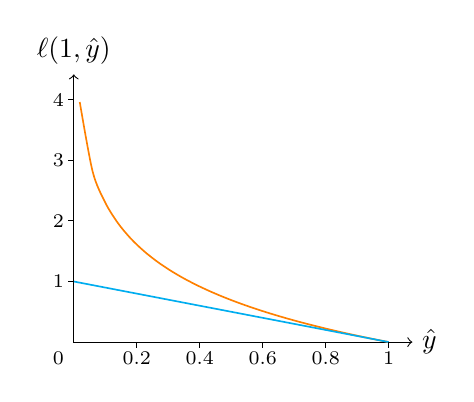
\begin{tikzpicture}

    \draw[<->] (4.3,0) node[right]{$\hat{y}$} -|(0,3.4) node[above]{$\ell(1,\hat{y})$};
    \draw[domain=0.019:1, semithick, smooth, orange] plot ({\x*4},{ln(1/\x)/1.3});
    \draw[domain=0:1, semithick, cyan] plot ({\x*4},{abs(1-\x)/1.3});

    \node[below left] at (0,0) {\scriptsize 0};
    %xticks
    \foreach \x in {0.2,0.4,...,1} {
        \draw (\x*4,0) -- (\x*4,-.07);
    }
    \node[below] at (0.2*4,0) {\scriptsize 0.2};
    \node[below] at (0.4*4,0) {\scriptsize 0.4};
    \node[below] at (0.6*4,0) {\scriptsize 0.6};
    \node[below] at (0.8*4,0) {\scriptsize 0.8};
    \node[below] at (1*4,0)   {\scriptsize 1};
    %yticks
    \foreach \y in {1,...,4} {
        \draw (0,\y/1.3) -- (-.07,\y/1.3);
    }
    \node[left] at (0,1/1.3) {\scriptsize 1};
    \node[left] at (0,2/1.3) {\scriptsize 2};
    \node[left] at (0,3/1.3) {\scriptsize 3};
    \node[left] at (0,4/1.3) {\scriptsize 4};

\end{tikzpicture}
    \end{subfigure}
    \caption{Confronto tra \textit{\color{cyan}absolute loss} e \textit{\color{orange}
    \label{fig:abs_vs_log}
    logarithmic loss}; a sinistra il caso $y=0$, a destra $y=1$.}
\end{figure}

Si noti in figura \ref{fig:abs_vs_log} come la \textit{logarithmic loss} tenda ad
infinito quando la predizione è opposta all'etichetta reale:
$$\lim_{\hat{y}\rightarrow 1^-} \loss(0,\hat{y})=\lim_{\hat{y}\rightarrow 0^+}
\loss(1,\hat{y}) = +\infty$$
In pratica questo previene 
l'utilizzo di predizioni $\hat{y}$ troppo sicure, quindi troppo vicine a zero o uno.

\subsection{Data domain \texorpdfstring{$\X$}{X}}
Verrà usata $\X$ per indicare l'insieme dei \textit{data points}; ogni suo punto $x \in \X$
è tipicamente un record di un database. Spesso un \textit{data point} può essere codificato 
come un vettore. Questa codifica risulta naturale in presenza di quantità omogenee, come i
pixel di un'immagine o una lista di occorrenze di parole in un testo. Quando invece i dati
presenti utilizzano unità di misura differenti, come \quotes{età} e \quotes{altezza}, la
codifica non risulta più immediata. Ci sarà bisogno di una procedura che codifichi i dati
in modo da ottenere uno spazio vettoriale omogeneo e coerente con i dati iniziali.
